\section{Differential test E1}
\label{sec:e1}

\subsection{Design}

E1 is a black-box differential test: the same inputs go into several programs written by different people, and the outputs are compared as printed. A plain scikit-learn 1.9.0 script (\code{scripts/oracle.py}) is the arbiter, so agreement with the arbiter is what the test measures; the arbiter itself is not assumed correct, and the three independent engines (R, Excel, AI Studio) are what give a disagreement its weight.

Two example datasets were shuffled once with a recorded permutation and split once into fixed train and test halves: the diabetes file into 353 and 89 rows, and the iris file into 120 and 30 rows. The split is written to disk (\code{data/}, with \code{md5sums.txt}) and every program reads the two halves as two tables; no program performs its own split, scaling, imputation, outlier handling, feature selection or hyperparameter search. A column named \code{order} carries the row identity and is excluded from the predictors everywhere.

Five cases were run. D1 and D2 are descriptive statistics of the two base files (n, mean, sample standard deviation, minimum, first quartile, median, third quartile, maximum; quartiles by the linear method that pandas, R type~7 and Excel \code{QUARTILE.INC} share). R1 is ordinary least squares on the diabetes training rows with ten predictors, compared on the intercept, the ten coefficients, the test RMSE, MAE and $R^2$, and all 89 test predictions. C1 is k-nearest neighbors on iris ($k=5$, Euclidean, uniform weights), compared on all 30 predicted classes. C2 is multinomial logistic regression on iris (L2, $C=1$, lbfgs, 100 iterations), compared on the 30 classes and the 90 class probabilities; R and AI Studio fit a differently regularized model and are excluded from C2 by plan, and Excel has no classifier.

DiGiTerra ran every case through its own routes (\code{/upload}, \code{/preprocess}, \code{/process}, \code{/export-bundle}, \code{/predict}) with the Advanced form's request, split method Time on the \code{order} column, test size 0.20, no scaler, seed 20260924 and ten decimal places. The other programs ran through their own interfaces: R 4.5.1 from a script, Orange 3.39.0 through its bundled Python, AI Studio 2026.0.1 from an imported process, Excel 16.03 from a workbook whose statistics and regression are Excel formulas (\code{COUNT}, \code{AVERAGE}, \code{STDEV.S}, \code{QUARTILE.INC}, \code{MEDIAN}, \code{LINEST}, \code{SUMXMY2}, \code{DEVSQ}).

\subsection{Controls}

Every program ran twice, with a close and reopen between runs, and the two saved outputs had to agree on every value. DiGiTerra ran R1 three times, twice at the start of the session and once at the end, and its predictions, coefficients and metrics files had to be byte-identical; only the run id, the timestamps and the artifact hash may differ. All controls passed for all five programs (\code{NOTEBOOK.txt}, entries marked CONTROLS PASS).

The comparison script (\code{scripts/compare.py}) formats every metric to \code{\%.6e} and classes each cell as \emph{same}, \emph{last digit} (mantissa differs by one unit in the last place), \emph{near zero} (both values within $10^{-12}$ of zero, which is where the centered diabetes columns land), \emph{rounded} (the value equals the arbiter rounded to a stated number of decimals), \emph{within $10^{-6}$}, or \emph{other}. The pass rule for a same-engine program (Orange, which runs scikit-learn) is zero \emph{other} cells and zero class mismatches; for an independent engine it is a relative difference below $10^{-6}$ on every value.

\subsection{Results}

Figure~\ref{fig:e1} counts every compared cell by program, case and class, from \code{RESULTS.csv} (2,436 cells after the 2026-09-25 completion). Figure~\ref{fig:e1r1} shows the relative differences behind the R1 bars, and Figure~\ref{fig:orange} the one set of cells classed \emph{other}.

\begin{figure}[htbp]
\centering
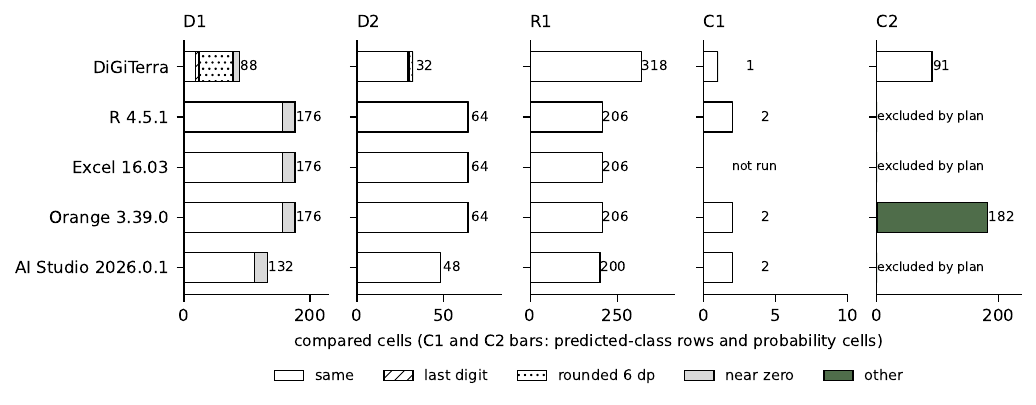
\includegraphics[width=\textwidth]{fig_e1_agreement}
\caption{E1 agreement by program and case. Each bar counts the compared cells; the fill marks the class. DiGiTerra's D1 and D2 bars carry \emph{rounded 6 dp} and \emph{last digit} cells because the application prints descriptive statistics to six decimals (a change made during the test; the original rounding was four). \emph{Near zero} cells are the ten centered diabetes means, which every program prints as a value within $10^{-16}$ of zero. Source: \code{docs/differential\_test\_E1/RESULTS.csv}.}
\label{fig:e1}
\end{figure}

\begin{figure}[htbp]
\centering
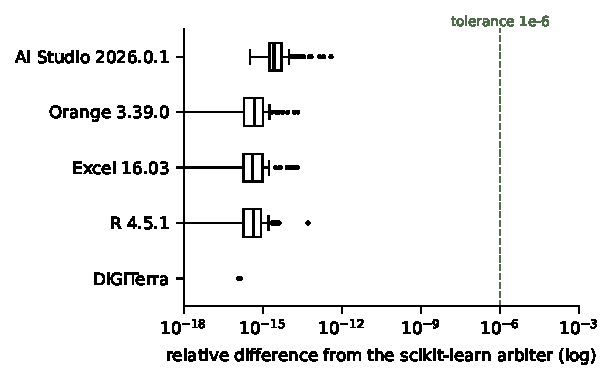
\includegraphics[width=0.6\textwidth]{fig_e1_r1_reldiff}
\caption{R1 ordinary least squares: relative difference from the arbiter for the intercept, the ten coefficients and the 89 test predictions, by program. DiGiTerra's cells are zero except three predictions at $1.4\times10^{-16}$ (one unit in the last place of the printed value); zeros are drawn at the axis floor. Every independent engine agrees with the arbiter to better than $10^{-12}$, six orders inside the $10^{-6}$ tolerance. Source: \code{RESULTS.csv}, case R1.}
\label{fig:e1r1}
\end{figure}

\begin{figure}[htbp]
\centering
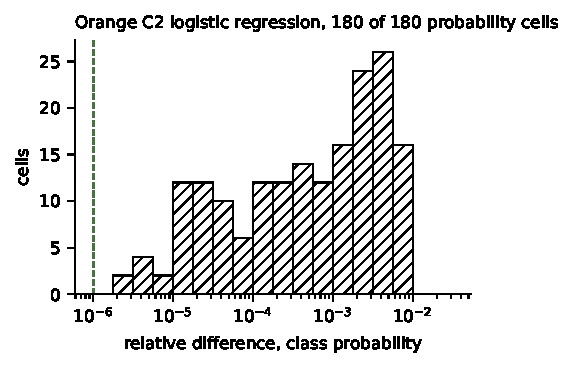
\includegraphics[width=0.6\textwidth]{fig_e1_orange_c2}
\caption{Orange C2: relative difference of the 90 class probabilities from the arbiter (180 cells over two runs). All 30 predicted classes agree; the probabilities differ by up to $7.9\times10^{-3}$. Source: \code{RESULTS.csv}, app orange, case C2.}
\label{fig:orange}
\end{figure}

R1 is the strongest result. The intercept, the ten coefficients and all 89 test predictions agree across DiGiTerra, R, Excel, Orange and the arbiter at six significant figures, and the largest relative difference on any R1 cell among the four reference programs is $3.8\times10^{-13}$ (AI Studio); R, Excel and Orange stay below $6\times10^{-14}$. DiGiTerra's own metrics differ from the arbiter by at most $3.6\times10^{-11}$ ($R^2$, printed to ten decimals). AI Studio agrees on the ten coefficients and the 89 predictions; its export omits the intercept, and its \code{squared\_correlation} is the squared Pearson correlation (0.5201965) rather than $R^2$ (0.5195044), which the plan anticipated, so $R^2$ was recomputed from AI Studio's own predictions and matches. C1 agrees on all 30 classes in every program that ran it. C2 agrees on all 30 classes in Orange, and DiGiTerra reproduces the arbiter's 90 probabilities exactly.

The Orange probability gap is the one open cell. Orange 3.39.0 bundles scikit-learn 1.5.2 on arm64. The same library version on x86\_64 gives the arbiter's probabilities (0.97462567 for the first row, not Orange's 0.97454283), a one-versus-rest fit gives 0.87, and a tight fit (tolerance $10^{-10}$, 116 iterations) differs from both. The remaining variable is the platform arithmetic under the loose default tolerance (arm64 Accelerate against x86\_64 OpenBLAS). That attribution is inferred, not established; it becomes established when \code{scripts/oracle.py} is run under Orange's own Python on the Mac and reproduces Orange's numbers. The \code{NOTEBOOK.txt} entry of 2026-09-24T17:40Z records the state.

Excel and AI Studio descriptive statistics were added on 2026-09-25 and completed the set. Excel's D1 and D2 agree on every one of the eight statistics for every column (156 cells same and 20 near zero for D1; 64 same for D2), and its R1 matches on 206 cells. AI Studio's Aggregate operator has no quartile function, so its D1 and D2 carry six statistics rather than eight (112 same and 20 near zero; 48 same). With those in place the comparison script reports the set as COMPLETE (\code{RESULT\_2026-09-25.txt}).

\subsection{What the test found in DiGiTerra}

Three defects were established in the version under test (tree \code{0942e0c}) and corrected before the results above were produced; the pre-fix outputs are kept in \code{digiterra\_outputs\_pre\_fix\_0942e0c/}. First, the regression metrics on the page and in the manifest were rounded to three decimals before the decimal-places setting was applied, so a setting of ten printed \code{53.8080000000} for a test RMSE of 53.808429803715498. Second, descriptive statistics were rounded to four decimals, so the diabetes means printed as $-0.0$. Third, for nineteen classifiers a hyperparameter typed on the Advanced form never reached the estimator while the run record still recorded the request; KNeighbors with \code{n\_neighbors} 3 was fitted with 5. The first two are closed by \code{tests/unit/test\_decimal\_setting.py} and the E1 rerun; the third by \code{test\_knn\_classifier\_form\_values\_reach\_the\_estimator} and the pass-through of form values for all nineteen. The third finding is the one a user could not have seen: the manifest said 3 and the model used 5.
